\documentclass{warpdoc}
\newlength\lengthfigure                  % declare a figure width unit
\setlength\lengthfigure{0.158\textwidth} % make the figure width unit scale with the textwidth
\usepackage{psfrag}         % use it to substitute a string in a eps figure
\usepackage{subfigure}
\usepackage{rotating}
\usepackage{pstricks}
\usepackage[innercaption]{sidecap} % the cute space-saving side captions
\usepackage{scalefnt}
\usepackage{amsbsy}
\usepackage{bm}
\usepackage{amsmath}

%%%%%%%%%%%%%=--NEW COMMANDS BEGINS--=%%%%%%%%%%%%%%%%%%%%%%%%%%%%%%%%%%
\newcommand{\alb}{\vspace{0.1cm}\\} % array line break
\newcommand{\mfa}{\scriptscriptstyle}
\newcommand{\mfb}{\scriptstyle}
\newcommand{\mfc}{\textstyle}
\newcommand{\mfd}{\displaystyle}
\newcommand{\hlinex}{\vspace{-0.34cm}~~\\ \hline \vspace{-0.31cm}~~\\}
\newcommand{\hlinextop}{\vspace{-0.46cm}~~\\ \hline \hline \vspace{-0.32cm}~~\\}
\newcommand{\hlinexbot}{\vspace{-0.37cm}~~\\ \hline \hline \vspace{-0.50cm}~~\\}
\newcommand{\tablespacing}{\vspace{-0.4cm}}
\newcommand{\fontxfig}{\footnotesize\scalefont{0.918}}
\newcommand{\fontgnu}{\footnotesize\scalefont{0.896}}
\renewcommand{\fontsizetable}{\footnotesize\scalefont{1.0}}
\renewcommand{\fontsizefigure}{\footnotesize}
%\renewcommand{\vec}[1]{\pmb{#1}}
%\renewcommand{\vec}[1]{\boldsymbol{#1}}
\renewcommand{\vec}[1]{\bm{#1}}
\setcounter{tocdepth}{3}
\let\citen\cite
\newcommand\frameeqn[1]{\fbox{$\displaystyle #1$}}

%%%%%%%%%%%%%=--NEW COMMANDS BEGINS--=%%%%%%%%%%%%%%%%%%%%%%%%%%%%%%%%%%

\setcounter{tocdepth}{3}

%%%%%%%%%%%%%=--NEW COMMANDS ENDS--=%%%%%%%%%%%%%%%%%%%%%%%%%%%%%%%%%%%%



\author{
  Bernard Parent
}

\email{
  bernparent@gmail.com
}

\department{
  Department of Aerospace Engineering	
}

\institution{
  Pusan National University
}

\title{
  Flux Discretization Schemes
}

\date{
  2017
}

%\setlength\nomenclaturelabelwidth{0.13\hsize}  % optional, default is 0.03\hsize
%\setlength\nomenclaturecolumnsep{0.09\hsize}  % optional, default is 0.06\hsize

\nomenclature{

  \begin{nomenclaturelist}{Roman symbols}
   \item[$a$] speed of sound
  \end{nomenclaturelist}
}


\abstract{
abstract
}

\begin{document}
  \pagestyle{headings}
  \pagenumbering{arabic}
  \setcounter{page}{1}
%%  \maketitle
  \makewarpdoctitle
%  \makeabstract
  \tableofcontents
%  \makenomenclature
%%  \listoftables
%%  \listoffigures


\section{First-Order Schemes}

Consider the following system of conservation laws:
%
\begin{equation}
\frac{\partial U}{\partial t}+ \frac{\partial F}{\partial x}=0
\end{equation}
%
where $F=F(U)$. We can discretize the latter in conservative form as follows:
%
\begin{equation}
\frac{U^{n+1}_i-U^n_i}{\Delta t}+ \frac{F_{i+1/2}-F_{i-1/2}}{\Delta x}=0
\end{equation}
%
where $F_{i+1/2}$ refers to the discretized flux at the interface located between node $i$ and node $i+1$.

\subsection{Flux Vector Splitting (FVS)}

The Steger-Warming flux vector splitting (FVS) \cite{jcp:1981:steger} flux at the interface can be written as:
%
\begin{equation}
F_{i+1/2}=F^+_{i} + F^-_{i+1} 
\end{equation}
%
where the positive and negative fluxes are defined as:
%
\begin{equation}
F^\pm= A^\pm U = L^{-1} \Lambda^\pm L U 
\end{equation}
%
where $L$ is the left eigenvector matrix of the convective flux jacobian $A\equiv\partial F/\partial U$ and $L^{-1}$ is the right eigenvector matrix of $A$.
Further, the positive and negative eigenvalues are defined as:
%
\begin{equation}
\Lambda^\pm = \frac{1}{2}\left( \Lambda \pm |\Lambda|\right)
\end{equation}
%

\subsection{Flux Difference Splitting (FDS)}

The Roe-Van-Leer flux difference splitting scheme (FDS) can be written as
%
\begin{equation}
F_{i+1/2}=\frac{1}{2} \left( F_i + F_{i+1}\right) - \frac{1}{2}|A|_{i+1/2}\left(U_{i+1}-U_i \right) 
\end{equation}
%
where the Roe matrix is defined as:
%
\begin{equation}
|A|\equiv L^{-1} |\Lambda| L
\end{equation}
%
For a perfect gas, a still contact discontinuity can be captured within one cell with no dissipation through the use of the Roe averaging \cite{jcp:1981:roe}:
%
\begin{align}
\rho_{i+1/2} &= \sqrt{\rho_i \rho_{i+1}} \alb
H_{i+1/2} &= \frac{\sqrt{\rho_i}H_i + \sqrt{\rho_{i+1}}H_{i+1}}{\sqrt{\rho_i}+\sqrt{\rho_{i+1}}} \alb
u_{i+1/2} &= \frac{\sqrt{\rho_i}u_i + \sqrt{\rho_{i+1}}u_{i+1}}{\sqrt{\rho_i}+\sqrt{\rho_{i+1}}}
\end{align}
%



\section{Second-Order Total Variation Diminishing (TVD)}


\subsection{Conditions for Positive Coefficients: Backward Stencil}

Consider a scalar conservation law in semi-discrete form:
%
\begin{equation}
\frac{u^{n+1}_i - u_i }{\Delta t} + a \frac{u_{i+1/2}-u_{i-1/2}}{\Delta x} =0
\end{equation}
%
Now, we aim to find an expression for $u_{i+1/2}$ that is second-order accurate. For $a>0$ this can be done through an upwinded stencil as follows:
%
\begin{equation}
u_{i+1/2} = u_i + \underbrace{\frac{1}{2} \left( u_i - u_{i-1} \right)}_{\textrm{second-order terms}}
\end{equation}
% 
Multiply the second-order terms by a limiter function:
%
\begin{equation}
u_{i+1/2} = u_i + \frac{1}{2} \phi_{i+1/2} \left( u_i - u_{i-1} \right)
\end{equation}
% 
Similarly for $u_{i-1/2}$:
%
\begin{equation}
u_{i-1/2} = u_{i-1} + \frac{1}{2} \phi_{i-1/2} \left( u_{i-1} - u_{i-2} \right)
\end{equation}
% 
Substitute the latter 2 equations in the semi-discrete equation:
%
\begin{equation}
\frac{\Delta x}{a\Delta t} u^{n+1}_i - \frac{\Delta x}{a\Delta t} u_i  
+ u_i + \frac{1}{2} \phi_{i+1/2} \left( u_i - u_{i-1} \right)
- u_{i-1} - \frac{1}{2} \phi_{i-1/2} \left( u_{i-1} - u_{i-2} \right) 
= 0
\end{equation}
%
with
%
\begin{equation}
\frameeqn{
0\le \phi_{i+1/2}\le 1
}
\end{equation}
%
Rearrange the last term in the former equation:
%
\begin{equation}
\frac{\Delta x}{a\Delta t} u^{n+1}_i - \frac{\Delta x}{a\Delta t} u_i  
+ u_i + \frac{1}{2} \phi_{i+1/2} \left( u_i - u_{i-1} \right)
- u_{i-1} - \frac{1}{2} \phi_{i-1/2} \frac{u_{i-1} - u_{i-2}}{u_{i} - u_{i-1}}(u_i-u_{i-1}) 
= 0
\end{equation}
%
Now for convenience define the ratio of successive gradients $r_{i-1}$ as:
%
\begin{equation}
r_{i-1} \equiv \frac{u_{i} - u_{i-1}}{u_{i-1} - u_{i-2}}
\label{eqn:ri}
\end{equation}
%
Thus:
%
\begin{equation}
\frac{\Delta x}{a\Delta t} u^{n+1}_i - \frac{\Delta x}{a\Delta t} u_i  
+ u_i + \frac{1}{2} \phi_{i+1/2} \left( u_i - u_{i-1} \right)
- u_{i-1} -  \frac{1}{2 r_{i-1}} \phi_{i-1/2}  (u_i-u_{i-1}) 
= 0
\end{equation}
%
Write in coefficient form:
%
\begin{equation}
c_i^{n+1} u^{n+1}_i = 
  c_i u_i  
+ c_{i-1} u_{i-1}
\end{equation}
%
with the coefficients equal to:
%
\begin{equation}
c_i^{n+1}=\frac{\Delta x}{a\Delta t}
\end{equation}
%
%
\begin{equation}
c_i=\frac{\Delta x}{a\Delta t} - 1 - \frac{1}{2} \phi_{i+1/2} + \frac{1}{2 r_{i-1}} \phi_{i-1/2} 
\end{equation}
%
%
\begin{equation}
c_{i-1}=\frac{1}{2} \phi_{i+1/2} +1 - \frac{1}{2 r_{i-1}} \phi_{i-1/2} 
\end{equation}
%
The coefficient $c_i^{n+1}$ is always positive. Thus, the other two coefficients must also be positive to obtain monotone solutions. The coefficient $c_i$ can be made positive through a small enough time step. Now impose positivity on the coefficient $c_{i-1}$:
%
\begin{equation}
\frac{1}{2} \phi_{i+1/2} +1 - \frac{1}{2 r_{i-1}} \phi_{i-1/2}  \ge 0
\end{equation}
%
Isolate $\frac{1}{2 r_{i-1}} \phi_{i-1/2} $:
%
\begin{equation}
\frac{1}{2 r_{i-1}} \phi_{i-1/2}  \le \frac{1}{2} \phi_{i+1/2} +1 
\end{equation}
%
Recalling that the range for the limiter function is of $0 \le \phi \le 1$, the most restrictive condition is when $\phi_{i+1/2}$ is equal to 0. Thus:
%
\begin{equation}
\frac{1}{2 r_{i-1}} \phi_{i-1/2}  \le 1 
\end{equation}
%
If $r_{i-1}$ is negative then:
%
\begin{equation}
\frac{1}{2} \phi_{i-1/2}  \ge r_{i-1} ~~~\textrm{for }r_{i-1}<0 
\end{equation}
%
But the latter is always satisfied because $\phi$ must be greater than 0. Thus, the only condition that matters is when $r_{i-1}$ is positive. Then:
%
\begin{equation}
\phi_{i-1/2}  \le 2 r_{i-1} ~~~\textrm{for }r_{i-1}>0
\end{equation}
%
or
%
\begin{equation}
\frameeqn{
\phi_{i+1/2}  \le 2 r_{i} ~~~\textrm{for }r_{i}>0
}
\label{eqn:positive_condition_2o}
\end{equation}
%






\subsection{Conditions for Positive Coefficients: Central Stencil}

Consider a scalar conservation law in semi-discrete form:
%
\begin{equation}
\frac{u^{n+1}_i - u_i }{\Delta t} + a \frac{u_{i+1/2}-u_{i-1/2}}{\Delta x} =0
\end{equation}
%
with $a>0$.
Now, we aim to find an expression for $u_{i+1/2}$ that is second-order accurate. 
We can write the flux at the interface as a combo of a first-order flux and a second-order contribution as follows:
%
\begin{equation}
  u_{i+1/2}=\left\{ \begin{array}{ll} 
u_{i} & \textrm{~~~first-order}\\
\frac{1}{2} u_{i} + \frac{1}{2} u_{i+1} & \textrm{~~~second-order}\\
\end{array}\right.
\end{equation}
%
or
%
\begin{equation}
  u_{i+1/2}= 
u_{i} + \psi_{i+1/2} \frac{1}{2} (u_{i+1}-u_{i})
\end{equation}
%
where $0\le \psi \le 1$.
But recall that:
%
\begin{equation}
r_{i} \equiv \frac{u_{i+1} - u_{i}}{u_{i} - u_{i-1}}
\end{equation}
%
Thus:
%
\begin{equation}
  u_{i+1/2}= 
u_{i} + \psi_{i+1/2} r_i \frac{1}{2} (u_{i}-u_{i-1})
\end{equation}
%
This has the same form as in the previous subsection but with $\psi_{i+1/2} r_i = \phi_{i+1/2}$. Thus, note that $\psi_{i+1/2}<1$ entails
%
\begin{equation}
\psi_{i+1/2} r_i< r_i
\end{equation}
% 
Or
%
\begin{equation}
\frameeqn{
\phi_{i+1/2} < r_i
}
\end{equation}
% 
Also, substituting $\phi_{i+1/2}$ by $r_i \psi_{i+1/2}$, the coefficient form in the previous subsection becomes:
%
\begin{equation}
c_i^{n+1} u^{n+1}_i = 
  c_i u_i  
+ c_{i-1} u_{i-1}
\end{equation}
%
with the coefficients equal to:
%
\begin{equation}
c_i^{n+1}=\frac{\Delta x}{a\Delta t}
\end{equation}
%
%
\begin{equation}
c_i=\frac{\Delta x}{a\Delta t} - 1 - \frac{1}{2} r_i \psi_{i+1/2} + \frac{1}{2 r_{i-1}} r_{i-1} \psi_{i-1/2} 
\end{equation}
%
%
\begin{equation}
c_{i-1}=\frac{1}{2} r_i \psi_{i+1/2} +1 - \frac{1}{2 r_{i-1}} r_{i-1} \psi_{i-1/2} 
\end{equation}
%
Consider the second coefficient and set it positive.
%
\begin{equation}
\frac{\Delta x}{a\Delta t} - 1 - \frac{1}{2} r_i \psi_{i+1/2} + \frac{1}{2 }  \psi_{i-1/2} >0
\end{equation}
%
 Say that $\psi$ should be such that it does not force an excessively small time step. Let's say that the maximum time step allowed should be at least half of the one specified by the CFL condition. Thus let's here set the condition on the time step as:
%
\begin{equation}
\frameeqn{
\frac{\Delta x}{a\Delta t}>2
}
\end{equation}
% 
Consider worst case when $\Delta x/a\Delta t$ is as small as possible (i.e., equal to 2), and substitute it in the former:
%
\begin{equation}
1 - \frac{1}{2} r_i \psi_{i+1/2} + \frac{1}{2 }  \psi_{i-1/2} >0
\end{equation}
%
The last term on the LHS is always positive and is independent of the others. Thus consider worse case when the last term on the LHS is zero:
%
\begin{equation}
   r_i \psi_{i+1/2}  <2
\end{equation}
%
or
%
\begin{equation}
\frameeqn{
   \phi_{i+1/2}  <2
}
\end{equation}
%


%
\begin{figure}[h]
 \begin{center}
   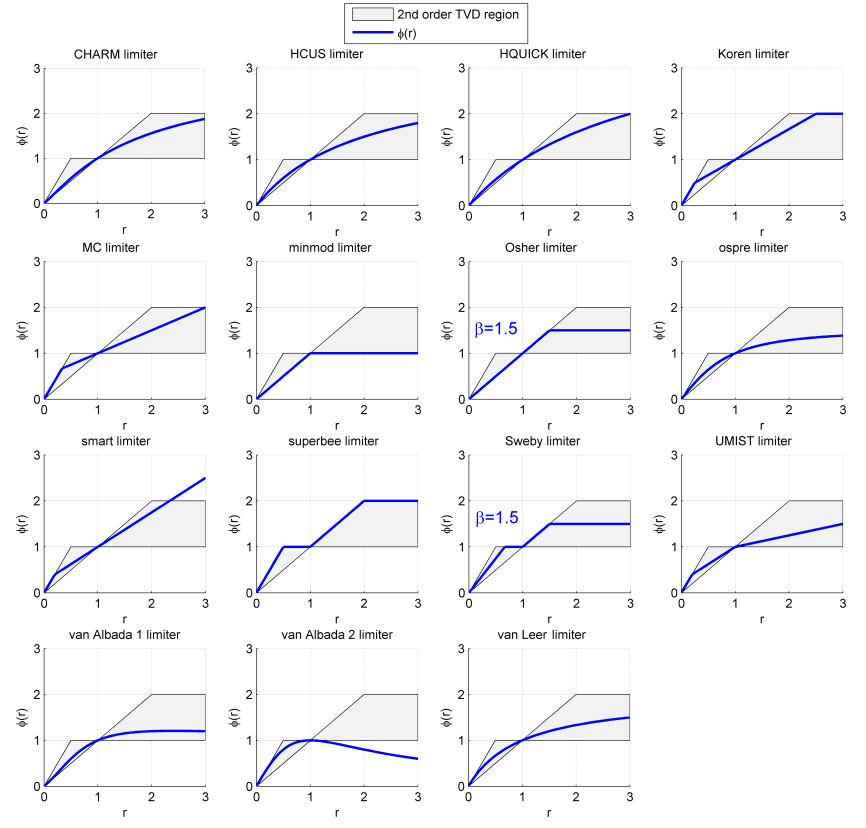
\includegraphics[width=5.9in]{LimiterPlots1.png}
 \end{center}
\caption{Limits of the TVD region as first shown by Sweby (1984). Courteousy of Wikipedia.}
\label{fig:TVD_limiter_region}
\end{figure}
%



\subsection{Summary of the Scheme}



The flux at the interface can be expressed as:
%
\begin{equation}
u_{i+1/2} = u_i + \frac{1}{2} \phi_{i+1/2} \left( u_i - u_{i-1} \right)
\end{equation}
% 
To adhere to the rule of the positive coefficients, the limiter should obey the condition (\ref{eqn:positive_condition_2o}):
%
\begin{equation}
\phi_{i+1/2}  \le 2 r_{i} ~~~\textrm{for~}  0 \le \phi_{i+1/2} \le 1
\end{equation}
%
with
%
\begin{equation}
r_{i} \equiv \frac{u_{i+1} - u_{i}}{u_{i} - u_{i-1}}
\end{equation}
%
To adhere to the rule of the positive coefficients, the limiter should also obey the following condition:
%
\begin{equation}
\phi_{i+1/2}  \le \min(r_{i},~2) ~~~\textrm{for~}  1 \le \phi_{i+1/2} \le 2
\end{equation}
%
As well, the limiter function should become 0 when the slope of the property changes sign:
%
\begin{equation}
\phi_{i+1/2}=0 ~~~\textrm{for~} r_i<0
\end{equation}
%
Such a region is referred to in the litterature as the second-order TVD region, as first proposed by Sweby \cite{sjna:1984:sweby}.
There are various limiter functions that satisfy all the above conditions, with the most popular ones being, arguably, the minmod, the superbee, \cite{arfm:1986:roe} and the Van Leer \cite{jcp:1974:vanleer} limiters:
%
\begin{equation}
\phi(r)= \left\{ \begin{array}{ll}
\max\left(0,~\min\left(1,~r\right)\right) & ~~~\textrm{minmod}\\
\max\left(0,~\min\left(1,~2r\right),~\min(r,2)\right) & ~~~\textrm{superbee}\\
(r+|r|)/(1+r) & ~~~\textrm{Van Leer}
\end{array}\right.
\end{equation}
%
The latter (and several other popular TVD limiter functions) are shown superimposed on the second-order TVD region in Fig.\  \ref{fig:TVD_limiter_region}.


\section{High Order Total Variation Diminishing (TVD)}

\subsection{Condition for Positive Coefficients}


Consider a scalar conservation law in semi-discrete form:
%
\begin{equation}
\frac{u^{n+1}_i - u_i }{\Delta t} + a \frac{u_{i+1/2}-u_{i-1/2}}{\Delta x} =0
\end{equation}
%
Now, we aim to find an expression for $u_{i+1/2}$ that is second-order accurate. For $a>0$ this can be done through an upwinded stencil as follows:
%
\begin{equation}
u_{i+1/2} = u_i + \underbrace{\left( u_{i+1/2}^{\rm ho} - u_i \right)}_{\textrm{high order terms}}
\end{equation}
% 
Multiply the second-order terms by a limiter function:
%
\begin{equation}
u_{i+1/2} = u_i +  \phi_{i+1/2} \left( u_{i+1/2}^{\rm ho} - u_i \right)
\end{equation}
% 
Similarly for $u_{i-1/2}$:
%
\begin{equation}
u_{i-1/2} = u_{i-1} + \phi_{i-1/2} \left( u_{i-1/2}^{\rm ho} - u_{i-1} \right)
\end{equation}
% 
Substitute the latter 2 equations in the semi-discrete equation:
%
\begin{equation}
\frac{\Delta x}{a\Delta t} u^{n+1}_i - \frac{\Delta x}{a\Delta t} u_i  
+ u_i + \phi_{i+1/2} \left( u_{i+1/2}^{\rm ho} - u_{i} \right)
- u_{i-1} - \phi_{i-1/2} \left( u_{i-1/2}^{\rm ho} - u_{i-1} \right) 
= 0
\end{equation}
%
Rearrange the two limited terms:
%
\begin{equation}
\frac{\Delta x}{a\Delta t} u^{n+1}_i - \frac{\Delta x}{a\Delta t} u_i  
+ u_i + \phi_{i+1/2} \frac{u_{i+1/2}^{\rm ho} - u_{i}}{u_{i+1}-u_i} (u_{i+1}-u_{i})
- u_{i-1} - \phi_{i-1/2} \frac{u_{i-1/2}^{\rm ho} - u_{i-1}}{u_{i} - u_{i-1}}(u_i-u_{i-1}) 
= 0
\end{equation}
%
Write in coefficient form:
%
\begin{equation}
c_i^{n+1} u^{n+1}_i = 
  c_i u_i  
+ c_{i-1} u_{i-1}
\end{equation}
%
with the coefficients equal to:
%
\begin{equation}
c_i^{n+1}=\frac{\Delta x}{a\Delta t}
\end{equation}
%
%
\begin{equation}
c_i=\frac{\Delta x}{a\Delta t} - 1 +  \phi_{i+1/2} \frac{u_{i+1/2}^{\rm ho} - u_{i}}{u_{i+1}-u_i}
 +  \phi_{i-1/2} \frac{u_{i-1/2}^{\rm ho} - u_{i-1}}{u_{i} - u_{i-1}}
\end{equation}
%
%
\begin{equation}
c_{i-1}=1 -\phi_{i-1/2} \frac{u_{i-1/2}^{\rm ho} - u_{i-1}}{u_{i} - u_{i-1}}
\end{equation}
%
The coefficient $c_i^{n+1}$ is always positive. Thus, the other two coefficients must also be positive to obtain monotone solutions. The coefficient $c_i$ can be made positive through a small enough time step. Now impose positivity on the coefficient $c_{i-1}$:
%
\begin{equation}
1 -\phi_{i-1/2} \frac{u_{i-1/2}^{\rm ho} - u_{i-1}}{u_{i} - u_{i-1}}\ge 0
\end{equation}
%
Or:
%
\begin{equation}
 \phi_{i-1/2} \frac{u_{i-1/2}^{\rm ho} - u_{i-1}}{u_{i} - u_{i-1}}\le 1
\end{equation}
%
If $u_{i-1/2}^{\rm ho} - u_{i-1}$ and $u_{i} - u_{i-1}$ don't share the same sign, then the condition becomes
%
\begin{equation}
 \phi_{i-1/2} \ge \textrm{negative number} ~~~{\rm for~}\frac{u_{i} - u_{i-1}}{u_{i-1/2}^{\rm ho} - u_{i-1}}\le 0
\end{equation}
%
Such is always satisfied because of the range of the limiter being $0 \le \phi \le 1$. If $u_{i-1/2}^{\rm ho} - u_{i-1}$ and $u_{i} - u_{i-1}$ share the same sign, then the condition becomes
%
\begin{equation}
 \phi_{i-1/2} \le \frac{u_{i} - u_{i-1}}{u_{i-1/2}^{\rm ho} - u_{i-1}} ~~~{\rm for~}\frac{u_{i} - u_{i-1}}{u_{i-1/2}^{\rm ho} - u_{i-1}}\ge 0
\end{equation}
%
or
%
\begin{equation}
\frameeqn{
 \phi_{i+1/2} \le \frac{u_{i+1} - u_{i}}{u_{i+1/2}^{\rm ho} - u_{i}} ~~~{\rm for~}\frac{u_{i+1} - u_{i}}{u_{i+1/2}^{\rm ho} - u_{i}}\ge 0
}
\label{eqn:positive_condition_ho}
\end{equation}
%





\subsection{Summary of the Scheme}

The flux at the interface can be expressed as:
%
\begin{equation}
u_{i+1/2} = u_i +  \phi_{i+1/2} \left( u_{i+1/2}^{\rm ho} - u_i \right)
\end{equation}
% 
where $u_{i+1/2}^{\rm ho}$ is a high-order representation of $u$ at the interface $i+1/2$. 
The first condition on the limiter condition is that it should be enclosed between 0 and 1:
%
\begin{equation}
  0 \le \phi_{i+1/2} \le 1
\end{equation}
%
Also, it should be such that it adheres to the rule of the positive coefficients, following condition (\ref{eqn:positive_condition_ho}):
%
\begin{equation}
 \phi_{i+1/2} \le \frac{u_{i+1} - u_{i}}{u_{i+1/2}^{\rm ho} - u_{i}} ~~~{\rm for~}\frac{u_{i+1} - u_{i}}{u_{i+1/2}^{\rm ho} - u_{i}}\ge 0
\end{equation}
%
As well, the limiter function should become 0 at extrema, i.e
%
\begin{equation}
\phi_{i+1/2}=0 ~~~\textrm{when~}\frac{u_{i+1}-u_i}{u_i-u_{i-1}}<0
\end{equation}
%
We can combine the latter 3 conditions with the expression for $u_{i+1/2}$ above to obtain:
%
\begin{equation}
\frameeqn{
 u_{i+1/2}=\left\{ 
\begin{array}{ll} 
u_i & \textrm{if~}\frac{u_{i+1}-u_i}{u_i-u_{i-1}}<0\alb
u_i+\min\left(u_{i+1}-u_i,~u_{i+1/2}^{\rm ho}-u_i\right) & \textrm{if~}\frac{u_{i+1}-u_i}{u_i-u_{i-1}}\ge 0\textrm{~and~if~}u_{i+1}-u_i>0\alb
u_i+\max\left(u_{i+1}-u_i,~u_{i+1/2}^{\rm ho}-u_i\right) & \textrm{if~}\frac{u_{i+1}-u_i}{u_i-u_{i-1}}\ge 0\textrm{~and~if~}u_{i+1}-u_i<0\\
\end{array}\right.
}
\end{equation}
%














\section{Weighted Essentially Non Oscillatory (WENO)}

The Essentially Non Oscillatory (ENO) method \cite{jcp:1987:harten} consists of choosing one of several high-order discretization stencils at the interface. To ensure that the solution remains non-oscillatory, the stencil chosen is the one that is the smoothest. How ``smooth'' a stencil can be defined in several ways, hence leading to a family of schemes. The Weighted Essentially Non Oscillatory (WENO) method \cite{jcp:1994:liu} consists of weighing the different stencils such that, in smooth regions, the order of accuracy of the resulting ``stencil mix'' is higher than the one of any of the stencils,  and in regions with discontinuities, the stencils that are the smoothest are given more weight than those who are not smooth.

We will here illustrate how to contruct a third-order accurate WENO using 2nd order accurate stencils as first proposed in \cite{jcp:1994:liu}. 
Say that we want to find the left and right states of $u$ at the interface between node $i$ and node $i+1$. For the left state, this can be done through a combination of one upwinded and one central stencil:
%
\begin{align}
  u_0&=\frac{3}{2} u_{i} -\frac{1}{2} u_{i-1} \alb
  u_1&=\frac{1}{2} u_i + \frac{1}{2} u_{i+1}
\end{align}
%
Now we wish to find a $u_{\rm L}$ at the interface that is third-order accurate and a combination of $u_0$ and $u_1$ as follows:
%
\begin{equation}
  u_{\rm L}=\gamma_0 u_0 + \gamma_1 u_1
\end{equation}
%
First, the optimal $u_{\rm L}$ should be third-order accurate. Thus the optimal $u$ at the interface should be:
%
\begin{equation}
u_{\rm L}=\frac{5}{6} u_i - \frac{1}{6} u_{i-1} + \frac{2}{6} u_{i+1}
\end{equation}
%
Substitute the former in the latter:
%
\begin{equation}
\gamma_0 u_0 + \gamma_1 u_1 
 = 
\frac{5}{6} u_i - \frac{1}{6} u_{i-1} + \frac{2}{6} u_{i+1}
\end{equation}
%
This gives one equation for two unknowns. The second equation is that the sum of the $\gamma$s must be one:
%
\begin{equation}
\gamma_0+\gamma_1=1
\end{equation}
%
From the latter two equations, we can easily show that:
%
\begin{align}
\gamma_0&=\frac{1}{3}\alb
\gamma_1&=\frac{2}{3}
\end{align}
%
The indicators of smoothness for each $u$ correspond to the square of the differences along each stencil:
%
\begin{align}
\beta_0&=(u_i-u_{i-1})^2 \alb
\beta_1&=(u_{i+1}-u_{i})^2
\end{align}
%
Then, $u_{\rm L}$ is made function of $u_0$ and $u_1$ with weights $w_0$ and $w_1$ multiplying $u_0$ and $u_1$ respectively:
%
\begin{equation}
 u_{\rm L}=w_0 u_0 + w_1 u_1
\end{equation}
%
with the weights defined as
%
\begin{align}
w_k = \frac{\tilde{w}_k}{\sum_l \tilde{w}_l} 
\end{align}
%
with
%
\begin{equation}
 \tilde{w}_k=\frac{\gamma_k}{(\epsilon + \beta_k)^2}
\end{equation}
%
with $\epsilon$ given a very small value.







\appendix


  \bibliographystyle{warpdoc}
  \bibliography{all}


\end{document}






